% Chapter 2
\documentclass[../main.tex]{subfiles}
\begin{document}

The model we have created apply methods well-known in the field of statistics, however using these methods to our model brings unique issues/decisions. In this chapter we will discuss these complications and explain and justify the decisions we make going forward. 

%% ISI distribution section.   
\section{ISI Distribution}

% Intro of the importance of the ISI distribution. What it involves and what it can inform us on. Why we care.
In this section we discuss the importance of the inter-spike interval (ISI) distribution. In Chapter 2 we gave an example whereby we created a time-dependent ISI distribution by extending the one dimensionial  Gamma$(\gamma, \gamma)$ distribution. The extension is performed by applying a time-rescaling method via the intensity function $x(t)$ which accounts for the time-dependence of \ce{Ca^2+} spiking. This approach can be used for a wide variety of probability distributions, such as an Inverse Gaussian or Weibull probability distributions. We will demonstrate that the choice of the original distribution is crucial to how well the model fits the \ce{Ca^2+} data. Furthermore, we will explain how to create a time-dependent ISI distribution from any probability distribution on $(0,\infty)$. Care is required in constructing these inhomogeneous ISI distributions to avoid non-identifiability issues. We will show how to circumvent this problem whilst also providing biological meaning to the intensity function used in creating these models. 

To begin, let us first consider the case of stationary \ce{Ca^2+} spikes --- spikes that depend only on the time since the last spike and not the time of the experiment. The ISI distribution can be modelled as a function of the time $t$ since the last spike $s$, whose domain is $(0,\infty)$. We can choose to model the ISI distribution $\psi (t,s)$ as a common probability distribution such as: an Exponential  
$$ \psi (t,s | \alpha ) = \alpha e^{-\alpha (t-s)},$$
  a Gamma
   $$ \psi(t,s| \alpha, \beta ) = \frac{\beta^\alpha \left( t-s\right)^{\alpha-1} e^{-\beta(t-s)}}{\Gamma(\alpha)},$$
   an Inverse Gaussian
   $$ \psi(t,s| \lambda, \mu) =\sqrt{\frac{\lambda}{2 \pi (t-s)^3}} \exp \left\{- \frac{\lambda((t-s)-\mu)^2}{2\mu^2(t-s)} \right\}, $$
   a Log Normal
   $$\psi(t,s| \mu, \sigma) = \frac{1}{(t-s)\sigma \sqrt{2\pi}} \exp \left\{- \frac{\left( (t-s)-\mu \right)^2}{2\sigma^2} \right\}, $$
 or a Weibull distribution
   $$ \psi(t,s | \lambda, k ) = \frac{k}{\lambda}\left( \frac{t-s}{\lambda}\right)^{k-1} e^{-\left( (t-s)/\lambda\right)^k}, $$
   
 where $\alpha$, $(\alpha, \beta)$, $(\lambda , \mu)$, $(\mu, \sigma)$ and $(\lambda, k)$ are the ISI parameters for each distribution, respectively. For a general distribution we denote the ISI parameters by $\theta$. Note that since we are considering stationary spikes, the distributions do not depend explicitly on the timing of spikes but the time since the last spike. This means the times $t$ and $s$ only appear as $t-s$ and we could rewrite $\psi(t,s| \theta) = \psi(t-s| \theta) = \psi(\tau| \theta) $, where $\tau$ denotes the time since the last spike.
 
 %Justification of each distribution
 We consider the Exponential distribution because it is the simplest distribution of $(0,\infty)$, moreover it describes a process which is memoryless, i.e. each spike is independent of all previous spikes. The Gamma distribution offers a natural extension to the Exponential distribution, such that the Exponential distribution is a special case of the Gamma --- where $\alpha = 1$. The Gamma distribution is an appealing candidate for the ISI distribution because it is a probability distribution for a combination of events occurring for the first time. Thus each event could be interpreted as a \ce{Ca^2+} puff, and each spike occurs the first time that $\alpha$ puffs occur.  
 	The Weibull distribution can also be viewed as an extension to the Exponential distribution --- the special case $k=1$ gives rise to the Exponential distribution. The Weibull distribution is often used to describe the ``time to failure'' of some component where the failure rate is proportional to a power of time. Thus, this distribution is justifiable if we believe \ce{Ca^2+} spikes depend on a power of time, i.e. if $k >1$ a spike is more likely to occur as time goes on. 
 	We use the Inverse Gaussian distribution because it has been used to model first passage events which contains positive drift and random drift only. Thus, since conceptually \ce{Ca^2+} spikes have been described as first passage events, the Inverse Gaussian is a suitable distribution to test. 
 	Finally, we also consider the  Log Normal because it is often used to model the firing rate across a population of neurons.  
 	 
% Add Gamma just and Inv Gauss just. 


%The IP distribution often serves as starting point for analysing spiking behaviour as it is the most basic statistical distribution. While the parsimony of the IP distribu- tion has undoubtedly helped in establishing a large body of mathematical results, real world data often exhibit more complex statistics. The IG distribution provides a natural extension of the IP distribution, in that it contains the IP distribution as a special case: putting γ = 1 in (5) recovers (10). The shape parameter γ endows the IG distribution with more flexibility, which has proven fruitful in numerous applications. Conceptually, spikes in general and Ca2+ spikes in particular have been described as first passage events [38]. One of the most fundamental models, which contains positive drift and random motion only, gives rise to the IIG distribution.

To find which of the models best describes a \ce{Ca^2+} spike sequence we first convert the spike sequence into a sequence of $M$ ISI times $\{T_i\}_{i=1}^M$. Then to fit the model $\psi(s|\theta)$ with ISI parameter/s $\theta$, we calculate the maximum likelihood estimate (MLE) $\hat \theta$  by 
$$\hat \theta  = \mathrm{arg max}_{\theta \in \Theta} \left\{ \prod ^M_{i=1} \psi(T_i | \theta ) \right\},$$
where $\Theta$ is the space of all possible parameter values. 

%Example using Ca spike sequence. 
To visualise the difference between the five stationary ISI distribution models we fit each model to the same spike sequence generated by a HEK293 cell challenged with $10\mu \mathrm{M}$ Carbachol. The cell exhibited 66 \ce{Ca^2+} spikes and we convert the spikes into a sequence of ISI times --- shown as the black ticks on the x-axis of Figure \ref{fig:ExampleISI}. Subsequently, we calculate the MLE for each of the distributions. The results are shown in the second column of Table \ref{table:Stationary}. We compare the models by examining the log likelihood at the MLE, shown as the third column in Table \ref{table:Stationary}. Superior models will have a higher log likelihood than other models. We find that the Exponential is the worst model having a log likelihood significantly lower than the other models. The Inverse Gaussian model has the largest log likelihood, implying it fits the spike sequence the best. However, the log likelihood of the Gamma is similar, thus either model could be used to describe the spike sequence.  

 To explain this difference in performance we plot the probability density function  of the MLE for each model. This is shown in Figure \ref{fig:ExampleISI} where dark green, orange, pink, light green and blue correspond to the Exponential, Gamma, Inverse Gaussian, Log Normal and Weibull distributions respectively. We see that the largest proportion of spike times are centered around 40s, which is mirrored by the probability densities of all the distributions bar the Exponential. The Exponential model does not capture this due to the limitations of its shape, i.e. it must take the shape of an exponential function. We see that the Gamma and Inverse Gaussian have similar probability density functions and hence similar likelihoods. Whereas, the Log Normal and Weibull have similar centers as the Gamma and Inverse Gaussian but with narrower and wider tails respectively. Zooming in on the region between 0s and 20s we see a single ISI just before 20s. In this region we see that the Weibull's probability density is too high --- we would expect more ISIs lower the 20s --- and the Log Normal's probability density is too low --- the density at the lowest ISI time is almost zero. This illustrates why the Log Normal and Weibull do not fit the ISIs as well as the Gamma and Inverse Gaussian models. 

% Table of fitting stationary distributions.
\afterpage{%
\clearpage
\begin{table}[t!]
  \begin{center}
    \begin{tabular}{|l|l|l|}
    \hline
     Distribution & MLE of ISI parameter/s & Log Likelihood  \\ \hline
     \cellcolor{col1} Exponential & $(\alpha) = 0.0221 $ & $-312.75$ \\ 
    \cellcolor{col2} Gamma & $(\alpha, \beta) = (0.229,10.35)$ & $-261.86$ \\
     \cellcolor{col4} Inverse Gaussian & $(\lambda,\mu) = ( 442.13, 45.22)$ & $-261.06$ \\
     \cellcolor{col5} Log Normal & $(\mu, \sigma) = (3.762,0.312)$ & $-268.78$ \\
     \cellcolor{col3} Weibull & $(k, \lambda) = (3.226, 50.41)$ & $-266.48$\\ \hline
    \end{tabular}
    \caption{The MLE and log likelihood of the MLE of each distribution fit to \ce{Ca^2+} ISIs from a HEK293 cell challenged with $10\mu \mathrm{M}$ Carbachol. The colour of the distribution matches the colour of the probability densities shown in Figure \ref{fig:ExampleISI}. }
    \label{table:Stationary}
  \end{center}
\end{table} 

 \begin{figure}[h!]
   \begin{center} 
    \subfloat{{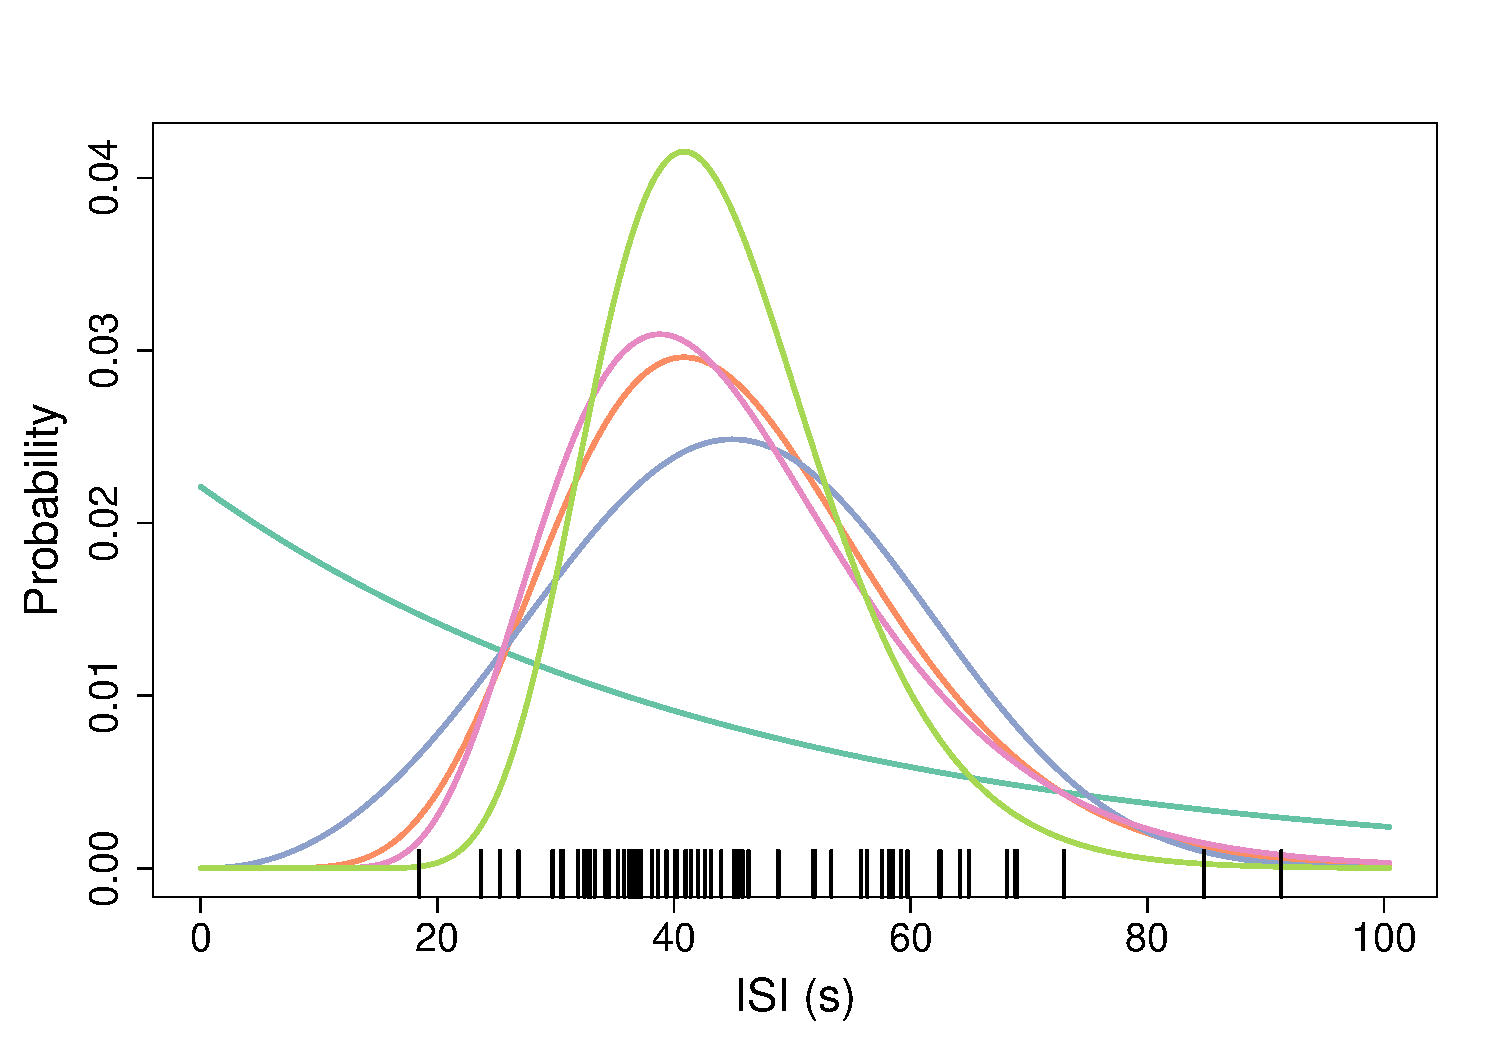
\includegraphics[width=0.8 \linewidth]{ISI_Stationary_plot} }}
    \end{center}     
    \caption{Probability density functions corresponding to the MLE of: an Exponential (dark green), a Gamma (orange), Inverse Gaussian (pink), Log Normal (light green) or Weibull Distribution (blue) fit to ISIs --- shown as black ticks on the x-axis.      }
    \label{fig:ExampleISI}
    \end{figure}
    \clearpage
}

%Summary of the stationary case. 
The above example demonstrates that the choice of ISI distribution is crucial, since we found that some distributions fit the \ce{Ca^2+} ISIs better than other distributions. This is due to the fact that shape of the probability density function varies for each family of probability distributions. Thus, when considering the ISI distribution for non-stationary spike sequences we need to consider several distributions as some may  describe the \ce{Ca^2+} spikes better than others.

%{\color{red} Worth mentioning other methods for stationary case? i.e could use non-parameter methods to estimate the ISI.}
%At this stage, one could argue to use a non-parametric method to estimate the ISI distribution. This would indeed be a more flexible framework since the ISI distribution would not be limited to the shape of the chosen probability distribution. 

%Back to our model.
Returning to our model, we want to create non-stationary ISI distributions by generalising the distributions --- the Exponential, Gamma, Inverse Gaussian, Log Normal and Weibull --- described in the stationary case above. 

% First the exponential distribution.
 et us begin with the Exponential distribution. This differs from the other considered distributions because it only has a single parameter $\alpha$. A point process with identical Exponential$(\alpha)$ ISI distributions is known as a Poisson process with rate $\alpha$ because the  number of events in the interval $[s,t]$ is a Poisson random variable with mean $\alpha (t-s)$. The non-stationary generalisation of the Poisson process is called an inhomogeneous Poisson process, where the parameter $\alpha$ is replaced with a rate function $\alpha(t)$. Thus, we shall call the inhomogeneous  Exponential ISI distribution
$$ p(t,s|\alpha) = \alpha(t) \exp \left\{ -\int^t_s \alpha(u) du \right\}. $$

%Other distributions - General.
 To generalise the distribution $\psi(t,s|\theta)$ we rescale time via the positive intensity function $x(t)$. This maps the original experiment time $r$ to a new time $z$ by
 $$ z(t) =\int^r_0 x(u) du. $$
 Thus by the transformation of variables we generalise the stationary ISI distribution $\psi(t,s|\theta)$ into a non-stationary ISI distribution $p(t,s| x, \theta)$ by
\begin{align*}
	p(t,s |x,\theta) &= \frac{dz}{dt} \psi (z(t),z(s)|\theta), \\
	&= \frac{dz}{dt} \psi (z(t) - z(s)|\theta),\\
	&= x(t) \psi (\int^t_0 x(u) du - \int^s_0 x(u) du|\theta), \\
	&= x(t)\psi (\int^t_s x(u)du|\theta),\\
	&= x(t)\psi (X(s,t)|\theta),
\end{align*} 
where $X(s,t) = \int^t_s x(u)du.$

We apply the transformation to the Gamma, Inverse Gaussian, Log Normal and Weibull distributions. We obtain the  inhomogeneous Gamma ISI
$$
 p(t,s| x, \alpha, \beta) =  \frac{\beta x(t)}{\Gamma ( \alpha )} \big[ \beta X(s,t) \big]^{\alpha -1} \exp \left\{ - \beta X(s,t)  \right\},
$$
 the inhomogeneous Inverse Gaussian
 $$
  p(t,s | x,\lambda, \mu) =  x(t) \bigg( \frac{\lambda}{2\pi X(s,t)^3} \bigg)^{0.5} \exp \left\{ -\frac{\lambda(X(s,t)-\mu)^2}{2 \mu ^2 X(s,t)} \right\},
 $$
 
 the inhomogeneous Log Normal 
 $$
  p(t,s| x, \mu, \sigma ) = \frac{x(t)}{X(s,t) \sigma \sqrt{2 \pi}} \exp \left\{ -\frac{(\log X(s,t) - \mu)^2}{2\sigma^2} \right\},
 $$
  
 and the inhomogeneous Weibull
$$
 p(t,s|x,k,\lambda) = \frac{x(t)k}{\lambda} \left( \frac{X(s,t)}{\lambda} \right)^{k-1} \exp \left\{ -\left( \frac{X(s,t)}{\lambda} \right)^k \right\}.
 $$
 Thus, each inhomogeneous ISI distribution has $x(t)$ as an additional parameter. The parameter set of the inhomogeneous Gamma, Inverse Gaussian, Log Normal and Weibull are $(x,\alpha,\beta)$, $(x,\lambda,\mu)$, $(x,\mu,\sigma)$ and $(x,k,\lambda)$ respectively.
     
% Non identifiability. 
We first need to check if each parameter in the ISI distribution is identifiable. This means that we can theoretically learn the true values of the parameters if given an infinite number of observations. Moreover, a model is non-identifiable if two distinct parameterisations lead to identical probability distributions. 

Begin by considering the Gamma ISI distribution. Notice that $\beta$ is always multiplied by either a factor of $x(t)$ or $X(s,t)$. Thus, it appears that we cannot untangle $\beta$ and the intensity function $x(t)$.  Indeed, consider the Gamma distribution with parameters $(ax,\alpha,\beta /a)$ with $a>0$ a constant, where we have varied the values of $\beta$ and $x$ but maintained the value of their product. Rearranging we get

 \begin{align*}
 p(t,s|ax, \alpha, \beta/a) &=  \frac{(\beta/a) ax(t)}{\Gamma ( \alpha )} \big[ (\beta/a) \int^t_s a x(u) du \big]^{\alpha -1} \exp\left\{ - (\beta/a) \int^t_s a x(u) du  \right\}, \\
 &=  \frac{\beta x(t)}{\Gamma ( \alpha )} \big[ (\beta/a) a\int^{t}_{s}  x(u) du \big]^{\alpha -1} \exp \left\{ - (\beta/a) a\int^{t}_{s}  x(u) du  \right\}, \\
  &=  \frac{\beta x(t)}{\Gamma ( \alpha )} \big[ \beta X(s,t) \big]^{\alpha -1} \exp\left\{ - \beta X(s,t)  \right\},\\
  &= p(t,s|x, \alpha, \beta).
 \end{align*}
Thus, we find two parameterisations with identical probability distributions and the Gamma ISI distribution is non-identifiable. Furthermore, all the other considered ISI distributions are also non-identifiable. This is shown in Table \ref{table:Non-ident}, where each distribution is given a pair of unique parameters that give rise to identical distributions --- for proof these parameter sets lead to identical distributions see Appendix {\color{red} XX}. 

%Maybe some line about the intensity replacing one of the parameters from the original distribution. 

% Table of Non-identifability
\begin{table}[h!]
  \begin{center}
    \begin{tabular}{|l|l|l|}
    \hline
     Distribution & Base parameters & Identical to ..  \\ \hline
     Gamma & $(x, \alpha, \beta)$ & $(a x, \alpha, \beta/a)$ \\
     Inverse Gaussian & $(x,\lambda,\mu)$ & $(a x, a\lambda, a \mu)$ \\
     Log Normal & $(x,\mu, \sigma)$ & $(a x, \mu + \log a, \sigma )$ \\
     Weibull & $(x, k, \lambda)$ & $(a x, k, a \lambda)$\\ \hline
    \end{tabular}
    \caption{Parameterisations of the inhomogeneous ISI distributions which lead to non-identifiability, where $a>0$ is a constant. }
    \label{table:Non-ident}
  \end{center}
\end{table} 

To resolve the non-identifiability issues we need to constrain the ISI distributions. One method for doing this is restricting the stationary distributions we used to create the inhomogeneous ISI distributions. For example we could restrict the stationary Gamma distribution from two parameters $(\alpha, \beta)$ to one parameter $\gamma$ by setting $\alpha = \beta = \gamma $ or $\alpha =\gamma$ and $\beta =\gamma^2$. However, there are infinitely many possibilities for restricting the stationary ISI distribution. Thus we want to find a clever way to restrict these distributions whilst giving meaning to the remaining parameters.   

Recall that the intensity function is a mathematical construct that allows time-dependent spiking processes to be factorised into individual ISIs. Thus, it would be advantageous to restrict the parameterisation in such a manner to give some meaning to the intensity function. Furthermore, it would be beneficial if the intensity function had the same meaning for each ISI distribution. In this case, after fitting, say, the Gamma and Inverse Gaussian model to \ce{Ca^2+} spikes we can check to see if intensity functions of both models are similar, which would show consistency between the models.   

Taking this into account, we choose to restrict the ISI distributions by setting the mean to one in the corresponding stationary ISI distributions. With this condition the intensity function coincides with the mean spike rate irrespective of the chosen stationary ISI distribution, i.e. Gamma, Inverse Gaussian, etc. 

% Example with Gamma to show how mean 1 = mean spike rate using histogramming. 
To visualise the impact of setting the mean of the stationary ISI distribution to one, we simulate spike sequences from a variety of inhomogeneous models. The intensity function $x(t)$ is the same for each model --- the red line in Figure \ref{fig:CompareHist}(A) and (B) --- and is drawn from a GP. The first model has a Gamma ISI distribution with parameters $\alpha = 1.8$ and $\beta = 1.8$, and the second model also has Gamma ISI distribution but with the parameters $\alpha = 3.6$ and $\beta = 1.8$. Recall that the mean of a Gamma distribution is $\alpha / \beta$, hence the mean for the first and second models are one and two respectively. We simulate 1000 spike sequences from both models and bin the spikes to calculate the mean spiking rate --- this is shown as the light and dark grey boxes in Figure \ref{fig:CompareHist}(A) for the first and second model respectively.  We find that only the spikes from the first model have mean spiking rate equalling the intensity function. In fact, the second model's mean spiking rate is equal to half the intensity function, shown as the red dotted line. Consequently, we find that only the Gamma ISI distribution with mean one has its mean spike rate coincide with the intensity function. 

%To visualisethe intensity function coinciding with the mean spike rate, we draw 1000 simulated spike sequences from two different models. Both models have the same intensity function --- solid red line in Figure \ref{fig:CompareHist}(A) --- and a Gamma ISI distribution. However, the parameters values of the Gamma distribution differs in each model with the first having parameters $(1.8,1.8)$ and the second $(3.6,1.8)$. Thus the first model's parameterisation has mean one whereas the second model has mean two. By binning the resultant spike times of each model we find the mean spike rate --- this is shown by the light and dark grey boxes for the first and second model respectively in Figure \ref{fig:CompareHist}(A). We find that for Gamma$(1.8,1.8)$ model the intensity distribution accurately describes the mean spike rate. However, the mean spike rate for the Gamma$(3.6,1.8)$ is half of the inputted intensity --- as shown by the dotted red line which is equal to half the intensity function. Thus by, fixing the mean of the original ISI distribution to one the intensity distribution describes the mean spiking rate. 

%Figure of comparing histograms with different parameterisations. 
     \begin{figure}[t]
    \begin{center}
	\begin{subfloat}{
	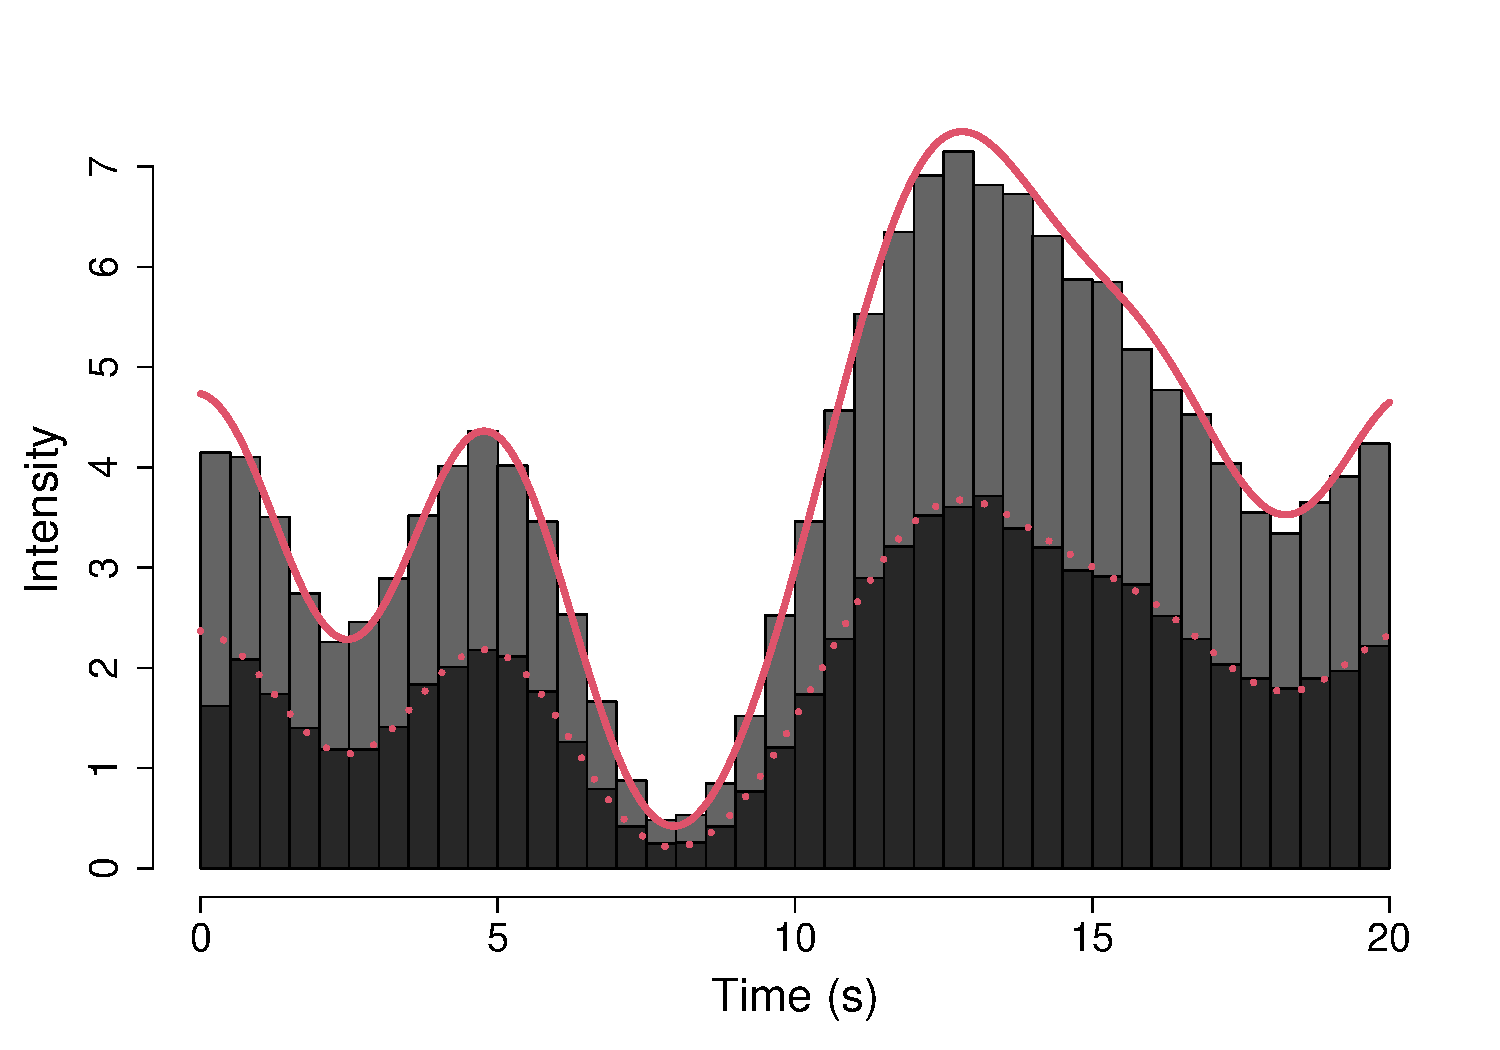
\includegraphics[width = 0.68\linewidth]{CompareHist}}
	\end{subfloat}
	\begin{subfloat}{
	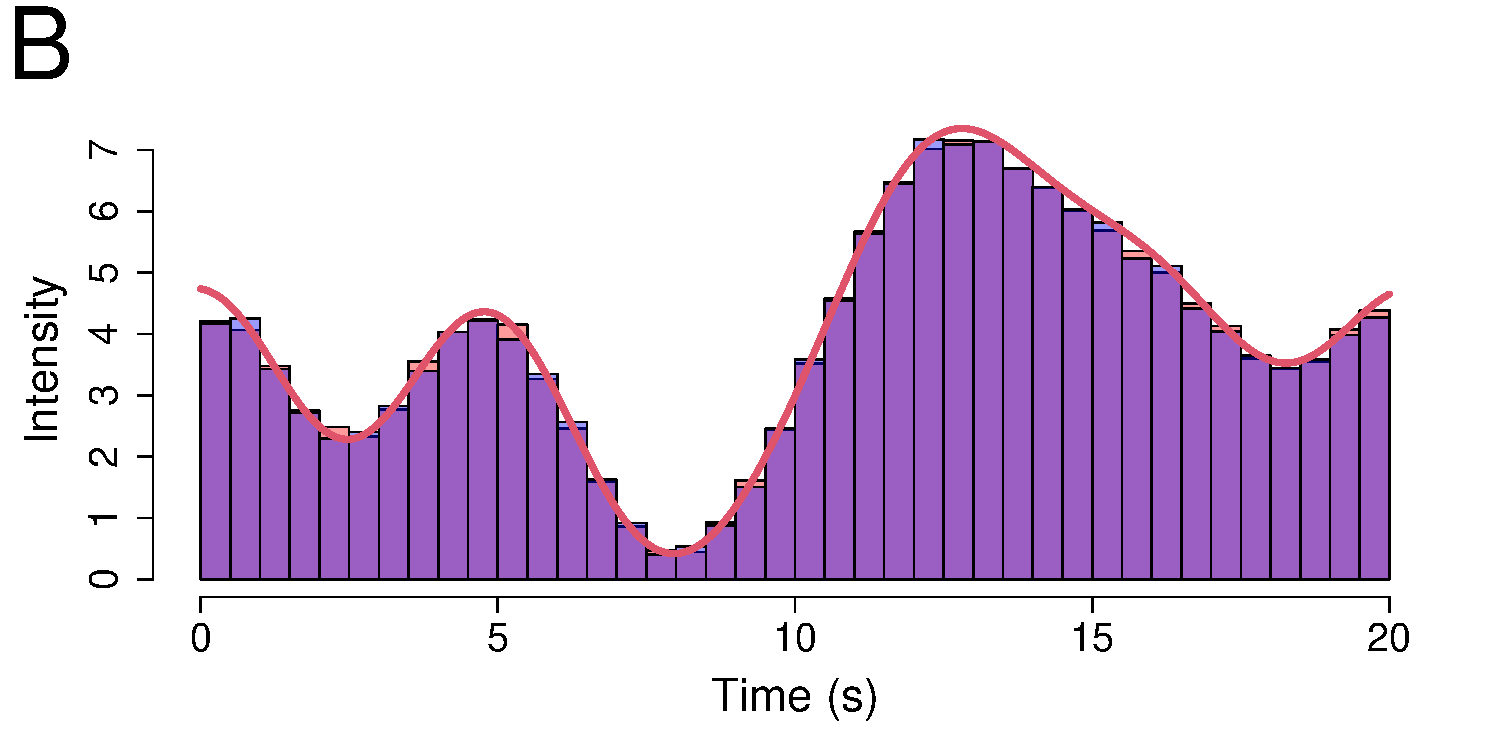
\includegraphics[width = 0.68\linewidth]{CompareHist_Dist}}
	\end{subfloat}	
		\caption{Comparing the intensity function --- the red line in both plots --- to histograms of 1000 simulated spike sequences. In (A) the light and dark boxes correspond to spikes generated from the model with Gamma ISI distributions with parameters Gamma(1.8,1.8) and Gamma(3.6,1.8) respectively. In (B) the spike sequences are simulated from a Gamma(1.8,1.8) and an Inverse Gaussian (1.8,1) resulting in the histograms in blue and red respectively, whose overlap is purple.  }
\label{fig:CompareHist}
\end{center}
\end{figure}


    
    
%Example to compare multi dists?
Furthermore, we consider a third model with the same intensity function but whose ISI distribution follows an Inverse Gaussian with parameters $\lambda=1.8$ and $\mu =1$, which has mean one. We simulate 1000 spike sequences from this model. In figure \ref{fig:CompareHist}(B), we compare the mean spike rate of this model with the first model ---  Gamma ISI distribution with mean one. The red and blue boxes correspond to binning the spike sequences from the Inverse Gaussian and Gamma models respectively. The overlap of the boxes is coloured purple. We see that the mean spike rate from both models are near identical. This shows that the intensity function of both models correspond to the mean spike rate, thus allowing us to compare intensity functions from models using different underlying probability distributions. 

%Furthermore, we can simulate 1000 spike sequences from the Inverse Gaussian ISI distribution with identical intensity function as above and parameters $(1.8,1)$, whose mean is one. In figure \ref{fig:CompareHist}(B) we compare the histograms of the simulated spike sequences from the Inverse Gaussian (red) and Gamma (blue) models, we see that the histograms are close to identical --- the overlap is coloured purple --- and the mean spike rate is the same for both models and equal to the intensity function. 

Henceforth, we use inhomogeneous ISI distributions generalised from stationary distributions with mean one, the parameterisations are shown in Table \ref{table:oneparam}. 

% Table of one-parameter distributions
\begin{table}[h!]
  \begin{center}
    \begin{tabular}{|l|l|l|}
    \hline
     Distribution & Original parameters & New parameter  \\ \hline
     Gamma & $(\alpha, \beta)$ & $(\gamma, \gamma)$, $\gamma >0$  \\
     Inverse Gaussian & $(\lambda,\mu)$ & $(\lambda, 1)$, $\lambda > 0$  \\
     Log Normal & $(\mu, \sigma)$ & $(-\mu, \sqrt{2\mu},)$, $\mu > 0$   \\
     Weibull & $(k, \lambda)$ & $(k,\frac{1}{\Gamma(1+1/k)})$, $k > 0$ \\ \hline
    \end{tabular}
    \caption{One parameter version of the stationary ISI distributions with mean one. }
        \label{table:oneparam}
  \end{center}
\end{table} 

Applying the time-rescaling transformation to the new restricted one-parameter version of the stationary distributions leads to the following inhomogeneous ISI distributions: the Gamma ISI distribution
$$
 p(t,s| x, \gamma) =  \frac{\gamma x(t)}{\Gamma ( \gamma )} \big[ \gamma X(s,t) \big]^{\gamma -1} \exp \left\{ - \gamma X(s,t)  \right\},
$$
 the Inverse Gaussian ISI distribution
 $$
  p(t,s| x,\lambda) =  x(t) \bigg( \frac{\lambda}{2\pi X(s,t)^3} \bigg)^{0.5} \exp \bigg\{-\frac{\lambda(X(s,t)-1)^2}{2 X(s,t)} \bigg\},
 $$
 
 the Log Normal ISI distribution
 $$
  p(t,s| x, \mu ) = \frac{x(t)}{2 X(s,t) \sqrt{\pi \mu}} \exp \left\{ -\frac{(\log X(s,t) + \mu)^2}{4\mu} \right\},
 $$
  
 and the Weibull ISI distribution
$$
 p(t,s|x,k) = \frac{x(t)k}{\frac{1}{\Gamma(1+1/k)}} \left( \frac{X(s,t)}{\frac{1}{\Gamma(1+1/k)}} \right)^{k-1} \exp \left\{ -\left( \frac{X(s,t)}{\frac{1}{\Gamma(1+1/k)}} \right)^k \right\}.
 $$

Recall, we also have the Exponential ISI distribution giving rise to an inhomogeneous Poisson process. We can replace $\alpha(t)$ with $x(t)$ since both describe the mean spiking rate of the process. Thus the inhomogeneous Exponential ISI distribution is given by
$$
 p(t,s|x) = x(t) e^{-X(s,t)}.
 $$
 
 %Summary 
 Thus, we have created five inhomogeneous ISI distributions based on the Exponential, Gamma, Inverse Gaussian, Log Normal and Weibull probability distributions. The time-dependence of each distribution comes from the intensity function $x(t)$ which represents the mean spiking rate. All the ISI distributions bar the Exponential also have a single ISI parameter $(\gamma)$, $(\lambda)$, $(\mu)$ and $(k)$ for the Gamma, Inverse Gaussian, Log Normal and Weibull respectively. This parameter describes the shape/variance of the ISI distribution. 
 
 %How does ISI param change the simulated spikes.
 In Figure \ref{fig:ISIParam} we show how the ISI parameter affects simulated spikes for the Gamma ISI distribution. We simulate spike sequences from two Gamma ISI models with the same intensity function (Panel A), where the first has ISI parameter $\gamma = 3$ (Panel B) and the second has $\gamma = 20$ (Panel C). We see that the larger ISI parameter leads to more regular spiking. This corresponds to an ISI distribution whose mass is centered around the mean with small tails. 
 % the ISI distribution we will For example in the Gamma ISI distribution the larger $\gamma$ the more centered around the mean spike rate the ISI distribution is, i.e. the ISI times are concentrated on the mean value. In Figure \ref{fig:ISIParam} we show the affect of the varying ISI parameter. We simulate spike sequences from two Gamma ISI models with the same intensity function (Panel A), where one has ISI parameter $\gamma = 3$ (Panel B) and the other has $\gamma = 20$ (Panel C). We see that the larger ISI parameter leads to more regular spiking, which corresponds to a ISI interval which is closely centered to its mean.  
 
 %Figure ISI parameter
   \begin{figure}[t!]
   \hrulefill
   \begin{center} 
    \subfloat{{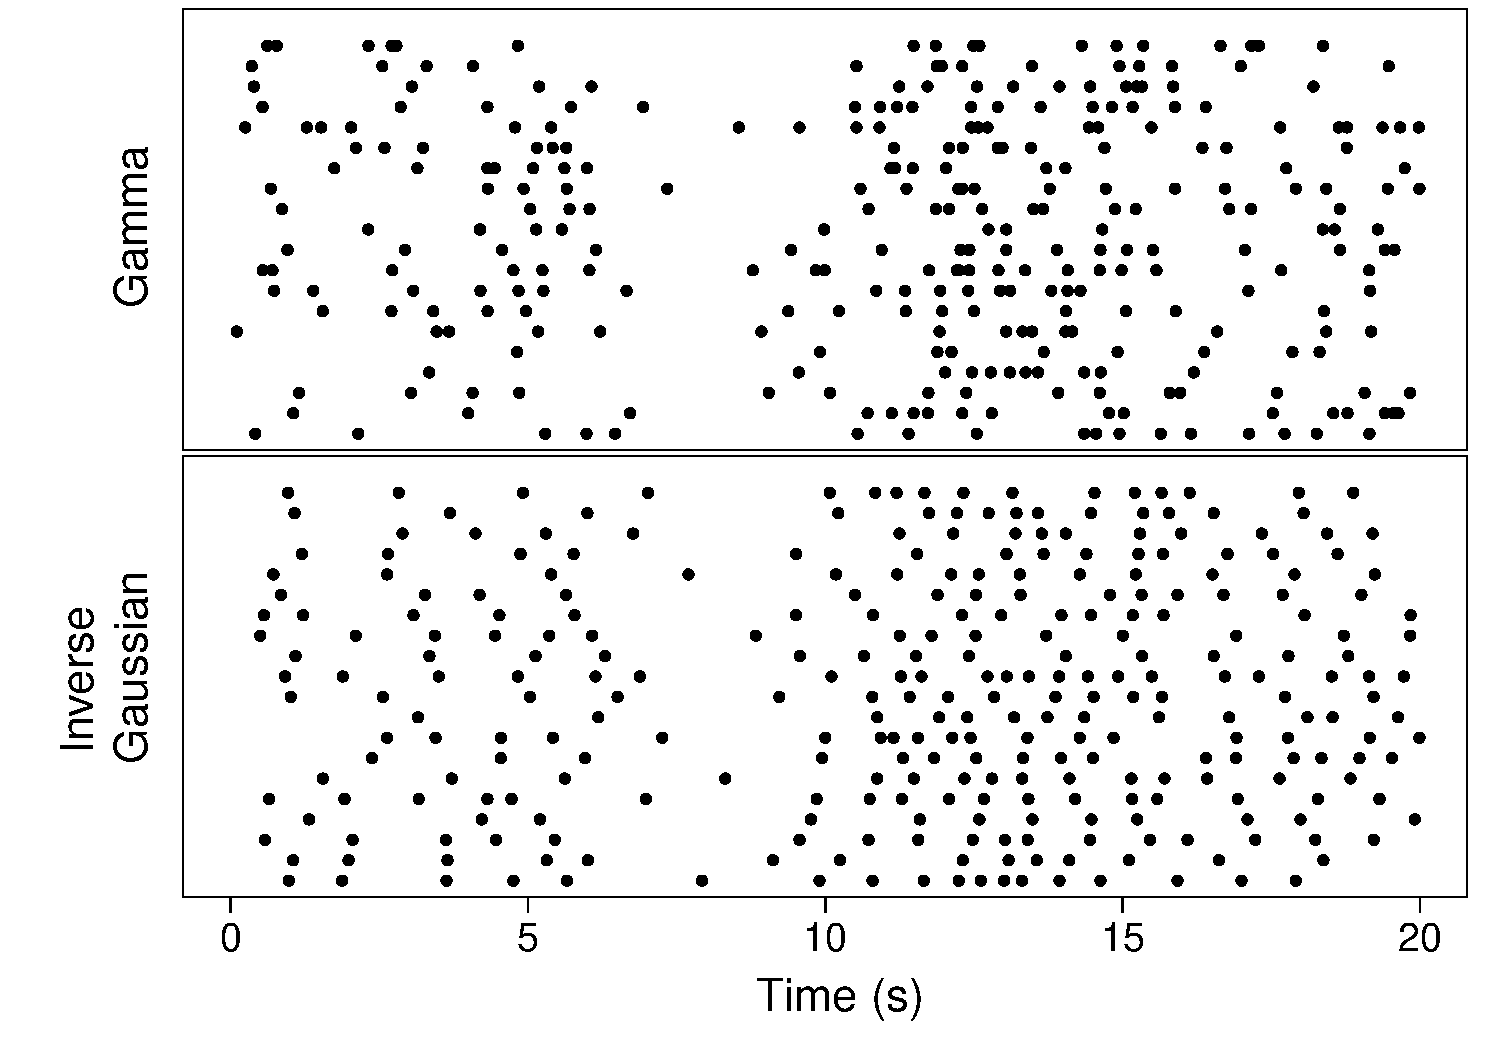
\includegraphics[width=0.8 \linewidth]{Image} }}
    \end{center}     
    \caption{Rastor plots comparing spike sequences drawn from two Gamma ISI distributions with the same intensity function ---  shown in (A) --- and differing ISI parameter. The sequences in  (B) and (C) correspond to $\gamma$ values of $3$ and $20$ respectively.}
    \label{fig:ISIParam}
    \hrulefill
    \end{figure}
 
 We will use the five ISI distributions --- namely Exponential, Gamma, Inverse Gaussian, Log Normal and Weibull  --- in our analysis of \ce{Ca^2+} spike sequences and explore which, if any, of the distributions best describe \ce{Ca^2+} data and what we can learn from the results.

%Paragraph on how these compare to previous work. 
%So now that we have decided on the ISI distributions we are going to apply, how do they relate to previous work? 

We now compare our inhomogeneous ISI distributions to previously explored distributions from the literature. 
Tilunaite et al [17]
%\cite{AGNE:1}
 used three ISI distributions in their work, the so-called inhomogeneous Poisson (IP), inhomogeneous Gamma (IG) and the inhomogeneous Inverse Gaussian (IIG). The IP and IG agree exactly with our Exponential ISI distribution and Gamma ISI distribution. However, their IIG ISI distribution has a different parameterisation to our Inverse Gaussian ISI distribution. Their model is generalised from the Inverse Gaussian with parameters $(1,\alpha)$ whereas our model is based on the parameters $(\lambda ,1)$. We do not use their parameterisation because the mean is not one, and as such the intensity function $x$ does not agree with the mean spiking rate. 

Thus the ISI distributions we consider builds upon previous work using the Exponential and Gamma ISI distributions and explores new distributions including the Log Normal and Weibull, which could better describe the \ce{Ca^2+} spike sequences.   

%It is important to note that although we may find that one probability distribution best describes the \ce{Ca^2+} spikes, there may exist a better untested model. In particular, in the above example if we only tested the Exponential, Log Normal and Weibull distribution we would have said that the Weibull distribution is the best candidate to describe the \ce{Ca^2+} spikes. Thus, we have shown that the choice of ISI distribution is vital when considering stationary models. 
\pagebreak

\section{Speed of the GP}
%Plan:
%	-Discussion of the MCMC algorithm and how the under-relaxed
In this section we discuss how a naive implementation of the GP prior in chapter 1 will lead to a computationally expensive algorithm. We will explain different methods to improve the algorithm, and justify our implementation.
 
In this framework we assume a priori that the intensity function $x(t)$ comes from a GP. To allow for computations we discretise time, often set to the frame rate of experimental data. Thus, the prior reduced to a multivariate normal distribution, over a large number of indexes, often greater then 1000 steps. To sample from the posterior intensity we utilise an under-relaxed method, where in each iteration we propose a candidate intensity $x_{\mathrm{can}}$ depending on the current value $x_{\mathrm{cur}}$ by
$$
x_{\mathrm{can}} = \sqrt{1-\omega^2} \log \left(x_{\mathrm{cur}} \right) +  \omega \nu , \qquad \nu \sim \mathcal{N}\left( \mathbf{0}, \Sigma \right)
$$ 

Thus, in each iteration we must generate a draw ($\nu$) from the multivariate normal distribution. This requires the inversion and determinant of the covariance matrix to be calculated, whose dimension is the discretisation chosen for the intensity, thus we need to be able to invert $1000 \times 1000$ matrices, quickly. There exists different methods to compute the matrix decomposition such as via eigenvalues?? or a choleski decomposition. However, these methods tend to be time consuming once the dimension increases. 

We have considered two different methods to improve the time taken, namely by implementing a projection when computing likelihoods and by expressing the GP by its spectral decomposition and simulating by a fast fourier transform (FFT). 

\subsection{Projection}
Explain how projection works.

\subsection{Spectral representation}
What is spectral density function? Define/explain.
In the case of a GP with 0 mean and squared exponential covariance function (write equation?) the spectral density is given by

$$
S(s) = \sigma^2 \left( 2 \pi \ell^2 \right)^{1/2}\exp \left( -2 \pi^2 \ell^2 s^2 \right) \cite{}
$$

However, not all kernels have a closed form for the spectral density, as such we can numerically calculate S via a FFT. Explain more. 

%However, in general we do not have a formula for the spectral density. We can numerically solve for S (if isotropic?? ) by:
%\begin{itemize}
%\item Find $t_{max}$ the value for which for all $ t > t_{max}$ we have cov$(t) < \epsilon$, for $\epsilon << 1$. (Choose $\epsilon = 1e-4$)
%\item create a grid $\mathbf{t}$ from $-t_{max}$ to $t_{max}$ in steps of size $\delta t$.
%\item compute S = (fftshift( fft( cov$(\mathbf{t})$)) $* t_{max}/Nt$) / $2 \pi$.
%\end{itemize}

Since A zero-mean GP is a real-values 1D-IV stationary stochastic process we can use the following theorem to express the gaussian process as an infinite series. 
{\it To every real-valued 1D-IV stationary stochastic process $f_0(t)$ with mean value equal to zero and two-sided power spectral density function $S_{f_0,f_0}(\omega)$, two mutually orthogonal real processes $u(\omega)$ and $v(\omega)$ with orthogonal increments $du(\omega)$ and $dv(\omega)$ can be assigned such that
$$
f_0(t) = \int^\infty_0 \left[\cos (\omega t)du(\omega) + \sin (\omega t)dv(\omega)  \right]
$$}



By the infinite series representation we can simulate the GP by the following series as $N \rightarrow \infty$
$$
f(t) = \sqrt{2}\sum^{N-1}_{n=0} A_n \cos(\omega_n t + \Phi_n)
$$
where
$$
A_n = \left( 2 S(\omega_n) \Delta \omega \right)^{1/2}, \qquad n=0,1,2,\dots,N-1
$$

$$
\omega_n = n\Delta \omega , \qquad n=0,1,2,\dots,N-1
$$

$$
\Delta \omega = \omega_c / N
$$

and

$$
A_0 = 0 \qquad \text{or} \qquad S(\omega_0 = 0) =0
$$

In equation - $\omega_c$ represents an upper cutoff frequency for which the spectral density is assumed to be zero for any larger frequency. To estimate $\omega_c$ we use the following criteria 
$$
\int^{\omega_c}_0 S(\omega) d\omega = \left( 1 - \epsilon \right) \int^{\infty}_0 S(\omega) d\omega
$$

To further improve the computation time we can rewrite this infinite series to a format which allows for the use of fast Fourier transform. Rewriting we get

$$
f(p \Delta t) = \Re \left( \sum^{M-1}_{n=0} B_n \exp \left[i (n\Delta \omega ) (p \Delta t) \right] \right)
$$
and $B_n$ 

The limitations of sampling from the GP in this method is that the step size, and number of steps is no longer independent. However, by choosing the value of M in a smart way we can still maintain the correct step size. Via 

\begin{algorithm}[t]
\DontPrintSemicolon
\textbf{Input:}\text{$N$, $\delta t$, $k(t_1,t_2)$  }\\ 
\textbf{Output:}\text{ Draw from GP }\\
\vspace{0.3cm}
Set $t=0$, $y_{\mathrm{cur}} = 0$, $\mathbf{y} = \oldemptyset$ and $h = T/K$; \;
\While{$t < T$}{
	Draw $a \sim U(0,1)$ and set $C = 0$; \;
	\While{$C< a$}{
	$t = t+h$; \;
	\If{$t > T$}{
	STOP; \;
	}
	Numerically calculate $C$ $= \int^t_{y_{\mathrm{cur}}} p(y_{\mathrm{cur}}, u |x(u), \theta ) du$; \;
	}
	Add $t$ to the set of spike times $\mathbf{y}$, and set $y_{\mathrm{cur}} = t$; \;
}
\textbf{Return} spike times $\mathbf{y}$; \;
\caption{Simulating Gaussian Process via spectral decomposition.}
\end{algorithm}


\section{Estimating Length Scale}
\begin{figure}[t]
	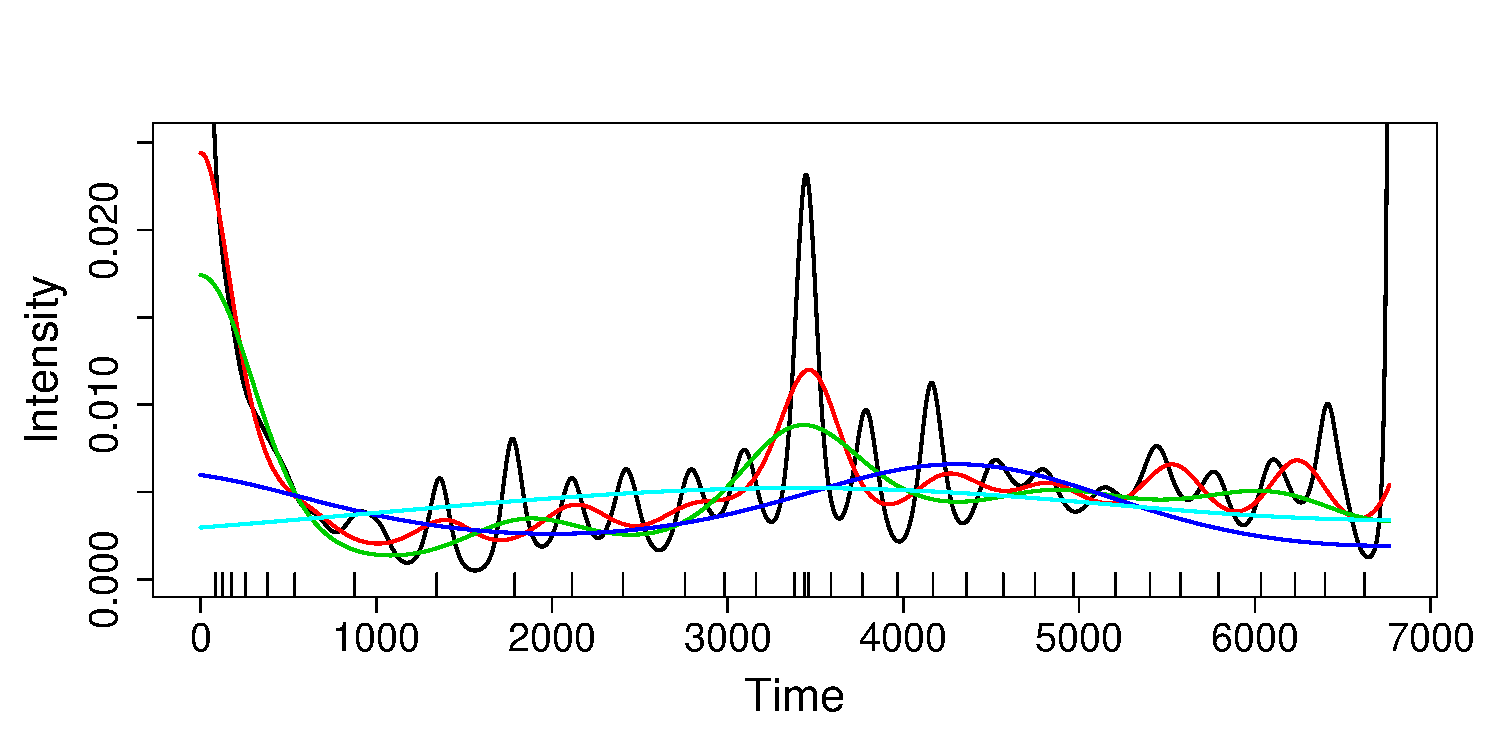
\includegraphics[width=\linewidth]{L_Estimate_Exs}
	\caption{Plot showing the mean posterior intensity functions with different fixed values of $l$, where the input data are the ticks on the x-axis.}
	\label{fig: LEstimate_EqualLikeli}
\end{figure}

For the GP prior there are three hyperparameters in the square exponential covaraince function, namely 
\subsection{How to estimate}
\subsection{Estimating with multiple data}
Suppose we now have several spike sequences corresponding to the same cell. We shall show that with simulated data that we can recover the all model parameters in this case. 

First we must choose the model we are going to use to generate the surrogate data. We take the experiment time to be $[0,30]$, then to choose an intensity function with a certain length scale we draw from a GP with the length scale taken to be 3. We further check the length scale of this intensity by estimating its value by an MCMC where the intensity is fixed and we calculate the posterior length scale. In figure \ref{fig: L_Estimate1} (A) we see the generated intensity which has been shifted by 1.4 so that the intensity is positive. In figure \ref{fig: L_Estimate1} (B) shows the trace plot for the posterior of $l$ given the intensity in (A) we see that this shows that the length scale for this function belongs in the interval $[5, 6.5]$. 

\begin{figure}
	\begin{subfloat}[]{
	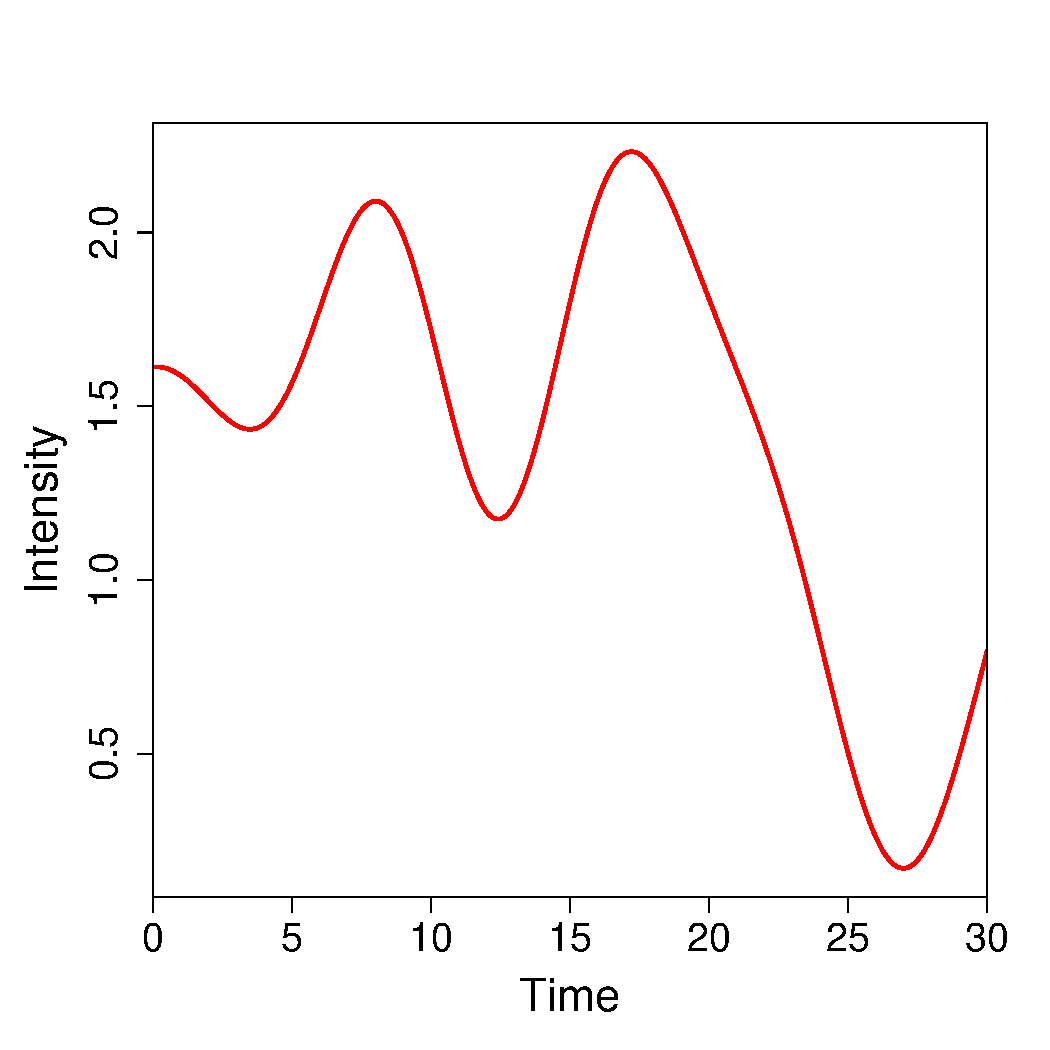
\includegraphics[width = 0.5\linewidth]{L_estimate_int}}
	\end{subfloat}
	\begin{subfloat}[]{
	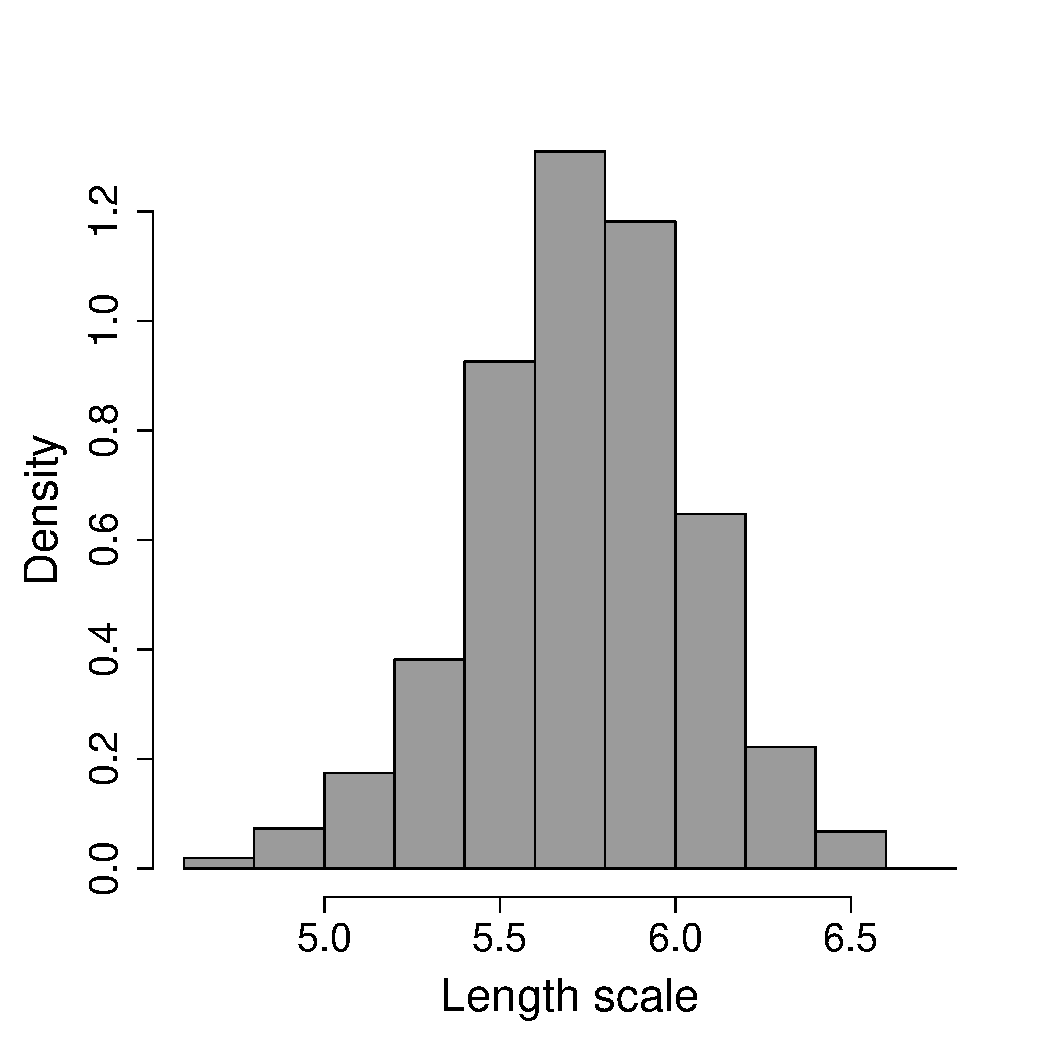
\includegraphics[width = 0.5\linewidth]{L_Estimate_lhist}}
	\end{subfloat}	
		\caption{(A) The intensity function drawn from a GP with mean 0 and length scale 3, used as the input to generate spike sequences. (B) Historgram of posterior samples of $l$ for the intensity function in (A). }
\label{fig: L_Estimate1}
\end{figure}

We now generate spike times from a model with the intensity described above. Furthermore, we set the ISI distribution to be a Gamma distribution with hyper parameter $\gamma = 7$. The results of the 20 simulated spike sequences can be seen in figure \ref{fig: L_estimate2}. We then use these spike sequences as an input into the MCMC algorithm where we assume that the intensity is apriori a GP. The posterior distribution is shown in figure \ref{fig: L_Estimate3}. Where the inputs to the algorithm were: iterations = 50000, burn = 20000, $\omega = 0.001$, the prior belief for $\gamma$ is exponential with rate 0.001, and the GP hyper parameters are set to $\sigma_f = 1000$ and $\sigma_n = 0.001$ with the RW metropolis for $\gamma$ and $l$ variance both set to 0.5. We see the posterior mean for $\gamma$ and $l$ are XX and XX respectively. This is close to the `true' values that the spikes were simulated from. Furthermore, we see in XX that the shape of the posterior intensity is similar to the inputted intensity. %Maybe more detail

From the above example we see that if we have several spike sequences for the same cell which can be inputted collectively then we can retrieve results very close to those that the spike sequences were simulated from. %Explain how this is better than if we only have one sequence.  
   
\begin{figure}
	\begin{subfloat}[]{
	\includegraphics[width = \linewidth ]{L_estimate1}}
	\end{subfloat}
	\begin{subfloat}[]{
	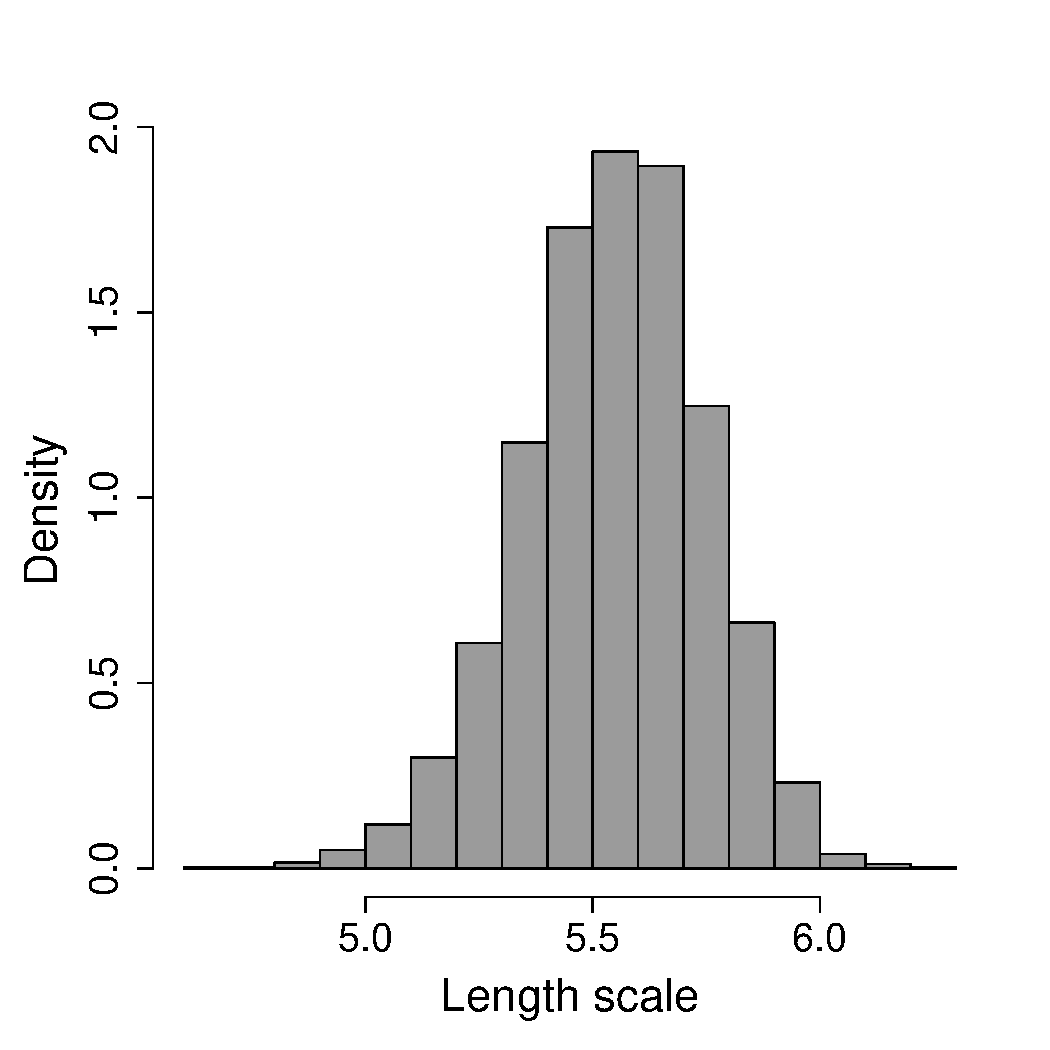
\includegraphics[width = 0.5\linewidth]{L_Estimate3}}
	\end{subfloat}
	\begin{subfloat}[]{
	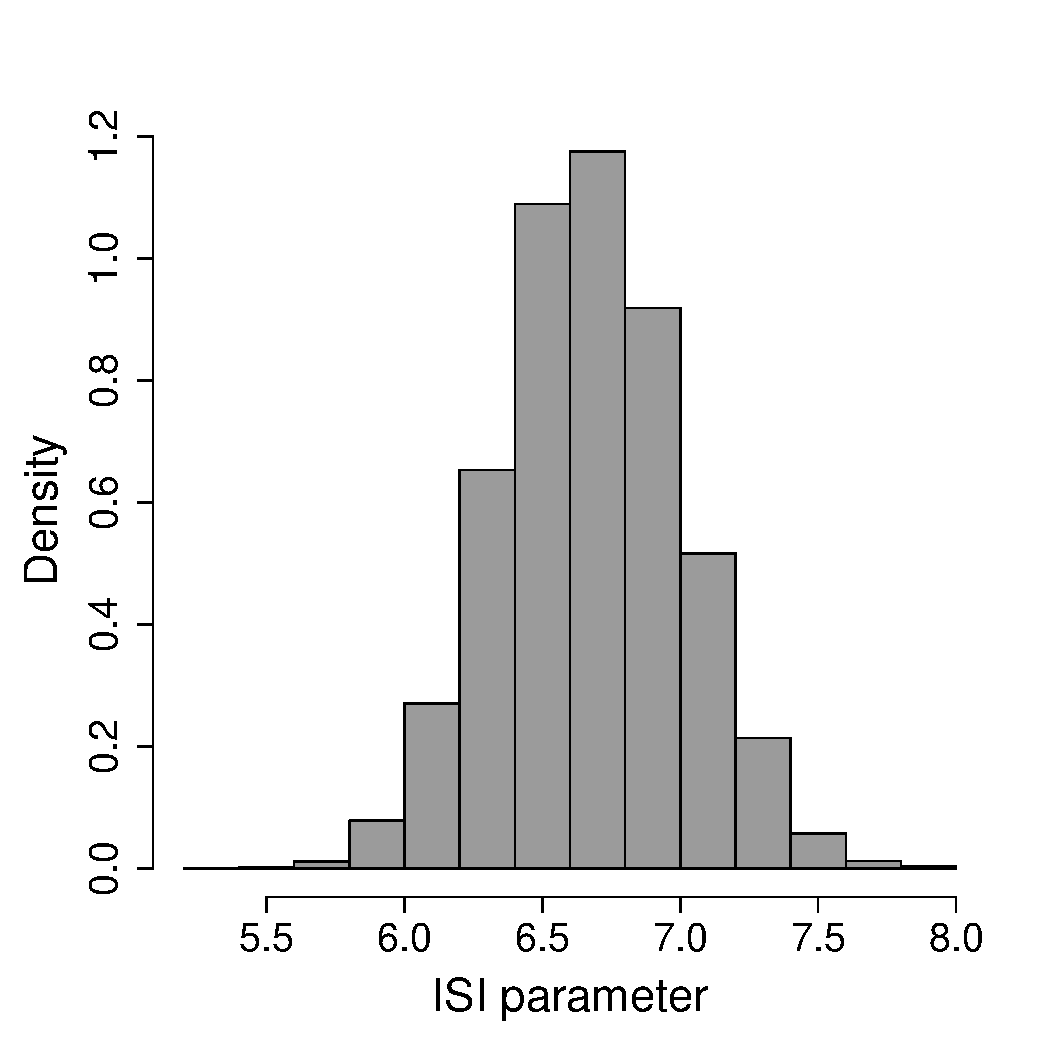
\includegraphics[width = 0.5\linewidth]{L_Estimate4}}
	\end{subfloat}	
		\caption{(A) The posterior intensity function (black) with 95\% confidence interval (grey), with the intensity function (red) that the spikes were drawn from. (B)(C) historgram of posterior for $l$ and $\gamma$ respectively. }
\label{fig: L_Estimate1}
\end{figure}


\subsection{Issues with single spike sequence}

\begin{figure}[t]
	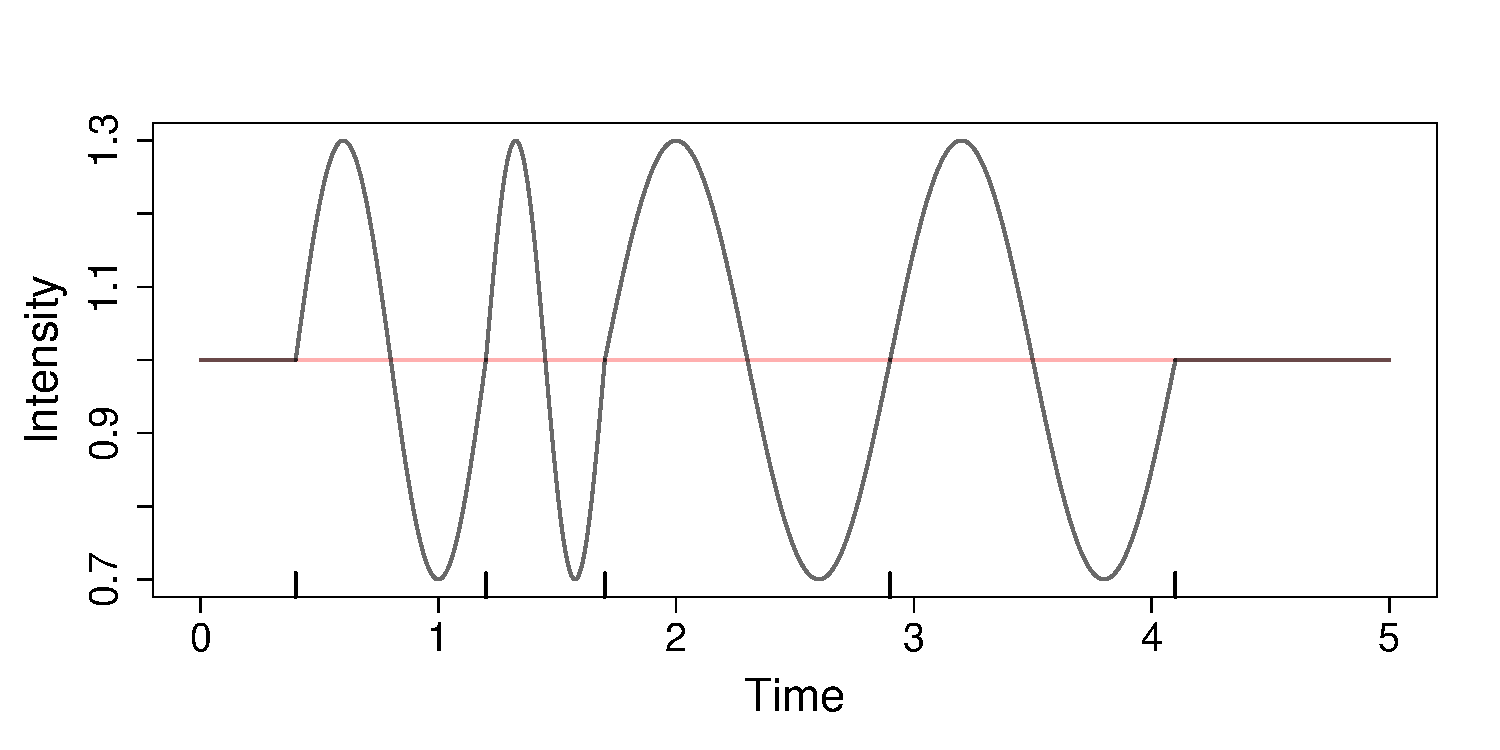
\includegraphics[width=\linewidth]{L_Estimate_SameLikeli}
	\caption{A plot show two intensities with different length scales, however both curves have the same integral between spike times and thus the same likelihood.}
	\label{fig: LEstimate_EqualLikeli}
\end{figure}


\end{document}
